% id: 99-21
% book: 100발100중 3-2 기말 · 01 3-2 기말(원의 성질·통계·부록)
% section: 실전 모의고사 3회
% figure: crop:fig-99-21.png
% answer: (1) $15^\circ$ (2) $9\mkern3mu \mathrm{cm}$
% answer_source: 답지(빠른정답)
% variant_level: 0 (원본 전사)
% 이 파일은 build.mjs 가 items.json 에서 만든다. 고칠 때는 items.json 을 고친다.
\smash{\raisebox{1.5mm}{\dmkichul{100발100중 3-2 기말 99쪽 21번 · 서술형}}}
\noindent\begin{minipage}[t]{0.58\linewidth}\vspace{0pt}\raggedright 그림과 같은 원에서 $\angle\pt{APB}=45^\circ$, $\angle\pt{CQD}=15^\circ$이고 $\arc{CD}=\arc{DE}=3\mkern3mu \mathrm{cm}$일 때, 다음 물음에 답하고, 그 과정을 서술하시오. \mbox{[5점]}\end{minipage}\hfill\begin{minipage}[t]{0.4\linewidth}\vspace{0pt}\centering 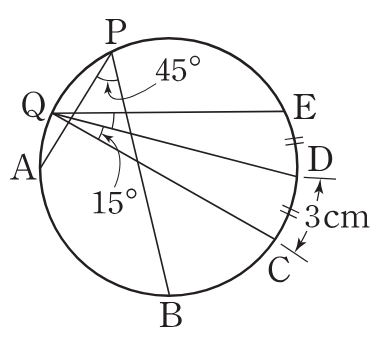
\includegraphics[width=90.8pt]{figures/fig-99-21.png}\end{minipage}\par
\dmsubprob{1} $\angle\pt{DQE}$의 크기를 구하시오. (2점)
\dmsubprob{2} $\arc{AB}$의 길이를 구하시오. (3점)
